\section{Implementazioni}
Il file system è stratificato, ogni livello si serve di funzioni dei livelli inferiori per realizzare funzioni utilizzate dai livelli superiori.

\begin{sitemize}
    \item \textbf{Dispositivi Hardware}
    \item \textbf{Controllo I/O:} Forniscono comandi che permettono di leggere specifiche locazioni di memoria del disco (leggi dal disco 1, cilindro 72, traccia 2, settore 10 nella locazione di memoria 1060) e li traducono in sequenze di bit che fanno spostare la testina alla locazione.

    \item \textbf{File System di Base:} Gestisce buffer e cache del dispositivo, fornisce comandi di più alto livello (leggi il blocco 123)
    \item \textbf{Modulo di organizzazione dei file:} Traduce indirizzi logici in indirizzi fisici
    \item \textbf{File System logico:} Gestisce le strutture dati del file system.
\end{sitemize}

\subsubsection*{Strutture Dati su Disco}
\begin{sitemize}
    \item \textbf{Blocco di controllo di avviamento:} O partizione di boot, contiene le informazioni necessarie all'avvio del disco, normalmente inizia dal primo blocco del disco.
    \item \textbf{Blocco di controllo dei volumi:} Contengono dettagli riguardo la partizione quali: numero dei blocchi (e dimensione), contatore blocchi liberi (e i loro puntatori)
    \item \textbf{Struttura delle directory}
    \item \textbf{Blocchi di controlli dei file:} Contengono i dettagli di ogni file quali: permessi, date (creazione, modifica), owner, dimensione, puntatore.

    NTFS utilizza una struttura dati in stile DB relazionale per queste informazioni.
\end{sitemize}

\subsubsection*{Strutture Dati su Memoria}
\begin{sitemize}
    \item \textbf{Tabella di montaggio:} Contiene informazioni su ogni volume montato
    \item \textbf{Struttura delle directory:} Una cache della struttura dati fisica.
    \item \textbf{Tabella dei file aperti}
    \item \textbf{Tabella dei file aperti per ciascun processo}
\end{sitemize}

\subsubsection*{ISO 9660}
Utilizzato dalle CD-ROM

\subsubsection*{UFS}
Unix File System, creato su il File System Berkley Fast (FFS)

\subsubsection*{Windows}
Supporta FAT, FAT32, FAT64, NTFS

\subsubsection*{Linux}
Fornisce ext2, ext3, ext4 (extended file system), ma supporta altri 40 tipi diversi.

\subsubsection*{GoogleFS}
Detto anche BigFiles è un file system ottimizzato per lo storage di file di grandi dimensioni (>100GB) con poche modifiche o eliminazioni.

\subsubsection*{OracleASM}
Gestisce file, directory, volumi grazie a direttive SQL.

\subsection{File System Virtuali}
Fornisce un'interfaccia comune per l'accesso a dispositivi con file system differenti.

\begin{figure}[H]
    \centering
    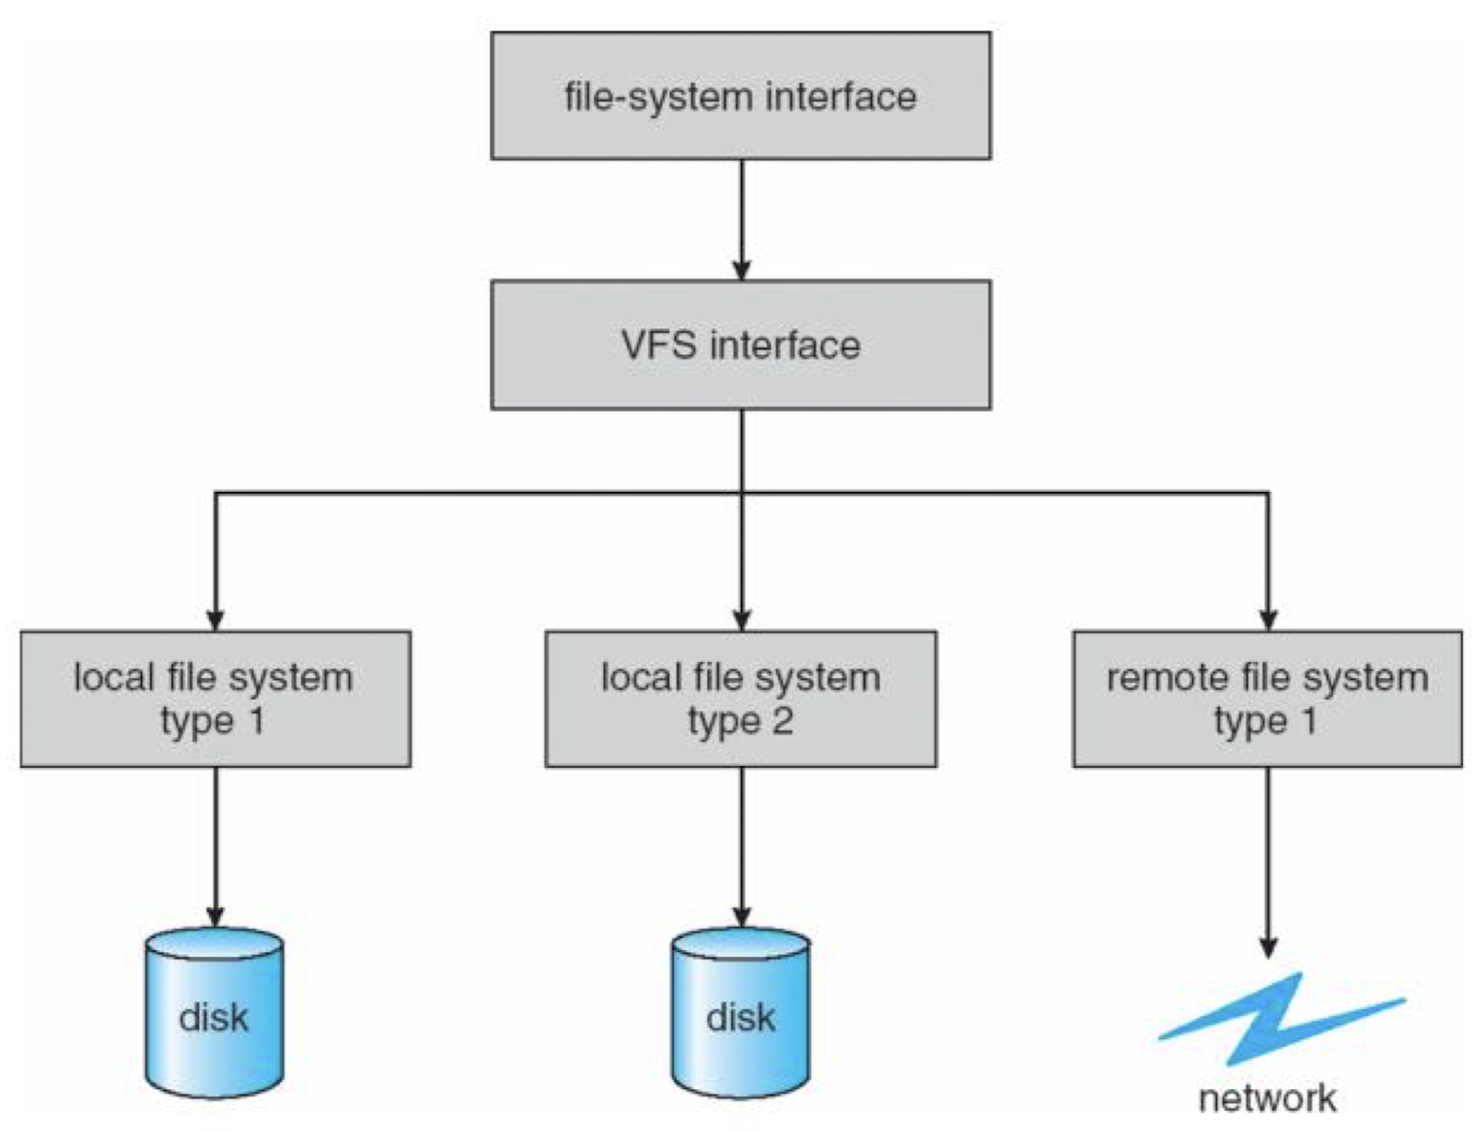
\includegraphics[width=0.5\linewidth]{assets/virtual-file-system.png}
\end{figure}

\subsection{NetWork File System}
Permette di unificare file system indipendenti di computer indipendenti nella rete, permette a qualsiasi utente di accedere al file system di qualsiasi altro computer.

In particolare rende possibile montare una directory remota specificando la posizione del calcolatore e quella del montaggio.

\begin{figure}[H]
    \centering
    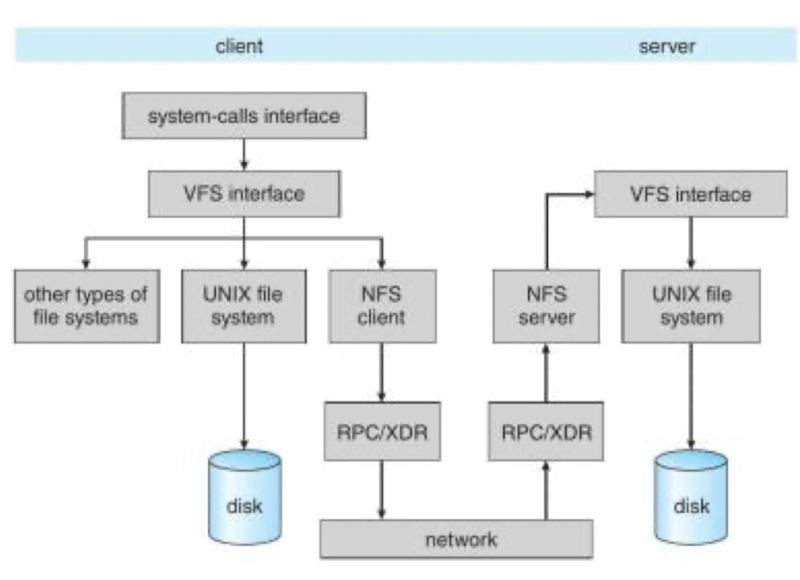
\includegraphics[width=0.5\linewidth]{assets/NFS.png}
\end{figure}

\subsubsection{FTP}
È possibile condividere file system anche attraverso la rete, il \textit{File Transfer Protocol (FTP)} permette di visualizzare ed accedere al file system di un altro calcolatore.

Questo è un modello client-server molti-a-molti, un server può gestire le richieste di più utenti ed un utente può accedere a molti server.
In questo caso per gestire l'autenticazione vengono utilizzate delle chiavi di cifratura, che introducono un'altra serie di complicazioni.

